% ─────────────────────────────────────────────────────────────────────────────
\section{Problem Statement}
\label{sec:intro-problem}

Booking recreational and informal services in Pakistan is a deeply fragmented and
inefficient process.  A customer who wants to reserve a futsal court for Friday
evening must: (1) find the vendor's WhatsApp number, (2) send a message asking for
availability, (3) wait for a manual reply---sometimes hours later, (4) negotiate a
time and price, (5) transfer an advance payment via JazzCash or bank transfer, and
(6) send a payment screenshot as confirmation.  If the chosen slot was taken by
another customer during the wait, the entire cycle restarts with a different vendor.

This friction is not limited to sports courts.  Salons, gaming zones, beach houses,
and most informal service businesses in Karachi operate identically.  No industry-wide
booking infrastructure serves this segment.  Existing digital solutions are narrow in
scope---sports-only apps or salon-specific platforms---and do not reflect the
cross-category, bilingual booking behaviour of real users.

A user survey conducted by the team in Spring 2025 ($n > 50$) quantified this
friction directly~\cite{survey2025}:
\begin{itemize}
  \item \textbf{72\%} of respondents rely on WhatsApp or phone calls to make bookings.
  \item \textbf{81\%} reported frustration with contacting multiple vendors to find
        an available slot.
  \item \textbf{68\%} said they would switch to an app that could handle the
        conversation and booking on their behalf.
\end{itemize}

Research by MoldStud~\cite{moldstud2024} corroborates that automated booking systems
``increase efficiency, reduce human error, and improve customer satisfaction.''
Kumar et al.~\cite{kumar2020} further show that structured digital workflows reduce
errors and missed reservations compared to manual methods.  Chatterjee et
al.~\cite{chatterjee2025} demonstrate through a Turf Booking System study that
real-time slot availability and automated conflict resolution improve both user
experience and vendor management---but their solution remains domain-specific and
does not extend to informal multi-category vendors or support autonomous agent-driven
negotiation.

At the vendor side, the problems mirror those of users.  Vendors manage incoming
WhatsApp requests across multiple simultaneous conversations, maintain schedules in
personal notebooks or Google Sheets, and face double-bookings whenever they are
offline or slow to reply.  Small vendors lack the resources to build dedicated booking
systems, causing them to miss revenue and to offer a poor customer experience.

The core computer science problem is therefore: \textit{how can an AI agent
understand and autonomously execute bilingual natural-language booking requests in
real time, while guaranteeing consistency in a distributed, multi-channel
environment?}  This decomposes into four sub-problems:

\begin{enumerate}
  \item \textbf{Bilingual NLU:} Parse booking requests in both English and Roman
        Urdu, handling code-switching (``Mujhe Friday ko 7 baje ke baad paddle court
        chahiye under 6000 rupees, preferably in defence'') and severe orthographic
        variation (\textit{waqt}, \textit{vakt}, \textit{wkht}, and \textit{tym} are
        all romanisations of the Urdu word for ``time'').
  \item \textbf{Dialogue Management:} Maintain conversation state across asynchronous
        WhatsApp sessions, handle partial information, manage clarification loops, and
        route user intent to the correct backend action.
  \item \textbf{Agentic Execution:} Autonomously check availability, hold slots
        atomically, verify payment proofs via OCR, and notify vendors---without
        hallucinating actions or bypassing business rules.
  \item \textbf{Concurrency Safety:} Prevent race conditions in a distributed NoSQL
        environment where multiple simultaneous requests may attempt to book the same
        time slot.
\end{enumerate}

% ─────────────────────────────────────────────────────────────────────────────
\section{Proposed Solution}
\label{sec:intro-solution}

\textbf{BookForMe} is a centralized, agentic AI-powered booking platform that
addresses all four sub-problems above.  It provides two complementary interaction
modes:

\begin{enumerate}
  \item \textbf{React Native Mobile App (Rich Client):} A full-featured mobile
        application that allows customers to browse vendors by category and location,
        view real-time availability calendars, select and confirm slots, upload
        payment proof, and access a social layer (matchmaking, forums, leaderboard).

  \item \textbf{WhatsApp AI Receptionist (Conversational Client):} An autonomous
        agent that operates on the vendor's existing WhatsApp Business number.
        Customers message the vendor in plain English or Roman Urdu; the agent
        understands their request, checks availability from the Firestore database,
        holds the slot via Optimistic Concurrency Control, requests a payment
        screenshot, verifies the amount via OCR, and notifies the vendor for final
        approval---all without requiring the vendor to participate in the conversation.
\end{enumerate}

Both clients share a single backend and database (the ``Single Source of Truth''),
meaning that a slot booked via WhatsApp is instantly reflected in the mobile app and
on the vendor dashboard.  Figure~\ref{fig:intro-overview} gives a high-level
overview of this architecture.

\begin{figure}[H]
  \centering
  \IfFileExists{images/introduction/system-overview.png}{
    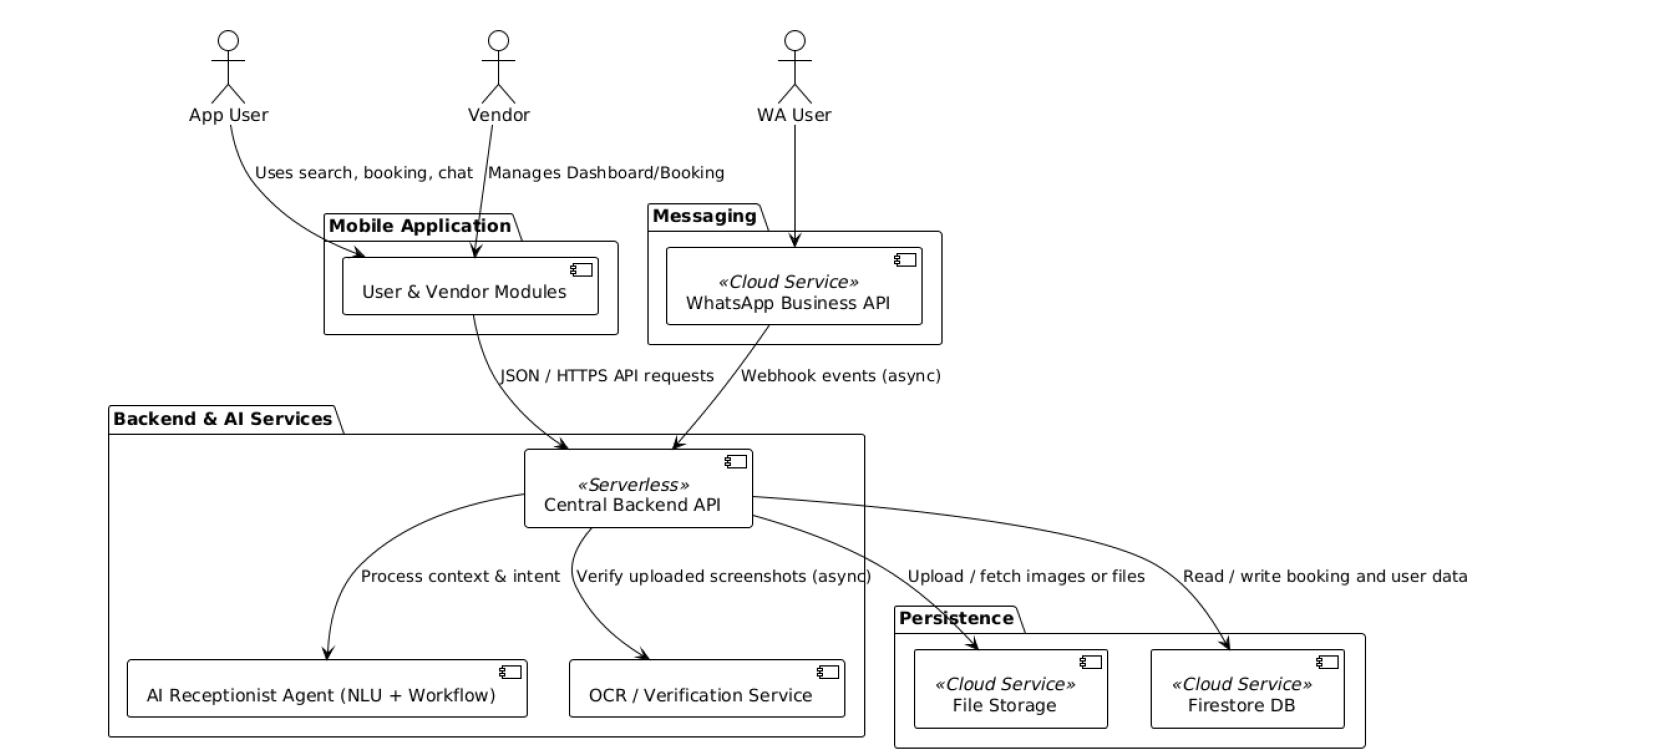
\includegraphics[width=0.9\textwidth]{images/introduction/system-overview.png}
  }{
    \fbox{\parbox{0.85\textwidth}{\centering\vspace{0.8cm}
    Missing figure file: \texttt{images/introduction/system-overview.png}\par
    System overview diagram placeholder\vspace{0.8cm}}}
  }
  \caption{High-level overview of the BookForMe platform.}
  \label{fig:intro-overview}
\end{figure}

What differentiates BookForMe from existing booking tools is the integration of
three capabilities within one platform:
\begin{itemize}
  \item bilingual NLU tuned to the local mix of English and Roman Urdu,
  \item a fully autonomous agentic workflow over WhatsApp with transactional safety,
  \item a social layer for player community and matchmaking across sports, salons,
        gaming zones, and other informal services.
\end{itemize}

% ─────────────────────────────────────────────────────────────────────────────
\section{Intended User}
\label{sec:intro-users}

BookForMe serves three distinct user groups:

\begin{description}
  \item[App Users (Customers)] Residents of Karachi who want to book informal
        services---predominantly sports-active young adults aged 18--35.  They
        interact with the platform primarily through the React Native mobile app,
        using the AI chatbot for natural-language search or manual browsing with
        filters for price, location, and amenities.  Social features (player matching,
        leaderboards, forums) are especially relevant to this group.

  \item[WhatsApp Users (Casual Customers)] Users who prefer not to install a
        separate app.  They interact exclusively through the vendor's existing
        WhatsApp Business number.  The AI Receptionist handles their entire booking
        journey---from availability check to payment confirmation---without requiring
        them to change their communication habits.

  \item[Vendors (Small Business Owners)] Owners of futsal courts, padel courts,
        salons, gaming zones, and similar informal services in Karachi.  They interact
        with BookForMe through the Vendor Dashboard, which provides a consolidated
        booking calendar (aggregating requests from the app and WhatsApp), analytics,
        pending-booking approvals, and an interface to link their WhatsApp Business
        account.  Crucially, vendors need no technical expertise---onboarding requires
        only connecting their WhatsApp number.
\end{description}

% ─────────────────────────────────────────────────────────────────────────────
\section{Project Gantt Chart and Deliverables}
\label{sec:intro-gantt}

Table~\ref{tab:gantt} shows the monthly project timeline across both Kaavish I
(CS~491) and Kaavish II (CS~492) semesters.

\begin{table}[!htbp]
\centering
\footnotesize
\caption{BookForMe project timeline and deliverables.}
\label{tab:gantt}
\setlength{\tabcolsep}{4pt}
\begin{tabularx}{\textwidth}{|l|X|X|}
\hline
\textbf{Month} & \textbf{Tasks} & \textbf{Deliverables} \\
\hline
\textbf{Sep--Oct 2025}
  \newline(Kaavish I)
  & Literature review; user survey; initial SRS; system architecture design;
    team role assignment; GitHub repository setup.
  & SRS v1; survey results; architecture diagram; project proposal. \\
\hline
\textbf{November 2025}
  & SRS v2 and SDS; initial bilingual dataset construction; low-fidelity UI wireframes;
    Firebase project and Firestore schema setup.
  & SRS v2; SDS; preliminary dataset (200 utterances); wireframes. \\
\hline
\textbf{December 2025}
  & Baseline NLU models (intent classification); Firestore CRUD APIs;
    React Native app skeleton (login, home, vendor listing).
  & Baseline NLU model; defined DB schema; minimal working booking system. \\
\hline
\textbf{January 2026}
  \newline(Kaavish II)
  & Fine-tune NLU pipeline; LangGraph agent implementation; WhatsApp webhook
    integration; OCC slot locking; OCR payment verification.
  & Functional AI Receptionist; WhatsApp-to-Firestore data flow; enhanced user dashboard. \\
\hline
\textbf{February 2026}
  & Vendor dashboard (calendar, analytics, booking approval); social features
    (matchmaking, forum, leaderboard, chat); model retraining and error analysis.
  & Full vendor dashboard; active social features; optimised bilingual NLU model. \\
\hline
\textbf{March 2026}
  & End-to-end integration; unit and integration testing; performance benchmarking;
    UX testing with real users; mid-evaluation presentation.
  & Fully integrated platform; test reports; benchmark metrics; mid-eval presentation. \\
\hline
\textbf{April 2026}
  & Pilot testing with selected Karachi vendors; production deployment on Firebase
    and Render; final documentation and report.
  & Production-ready deployment; final report; presentation deck; submission package. \\
\hline
\end{tabularx}
\end{table}

\noindent\textbf{Kaavish I Deliverables:}
\begin{itemize}
  \item Project proposal (approved)
  \item SRS v1 and v2
  \item Software Design Specification (SDS)
  \item Literature review
  \item Preliminary bilingual dataset
  \item Low-fidelity wireframes
\end{itemize}

\noindent\textbf{Kaavish II Deliverables:}
\begin{itemize}
  \item Functional AI Receptionist (WhatsApp agent, live demo)
  \item Full-stack React Native application (user app + vendor dashboard)
  \item Fine-tuned DistilBERT NLU model (90.5\% accuracy)
  \item OCR payment verification module
  \item Social features (matchmaking, forum, leaderboard)
  \item End-to-end test suite and benchmark results
  \item Production deployment (\url{https://jhat-to9p.onrender.com})
  \item This final report
\end{itemize}

% ─────────────────────────────────────────────────────────────────────────────
\section{Key Challenges}
\label{sec:intro-challenges}

\begin{description}
  \item[Roman Urdu Orthographic Variation]
        Roman Urdu lacks a standardised orthography.  A single word like
        \textit{waqt} (time) may appear as \textit{vakt}, \textit{wkht},
        \textit{waqat}, or \textit{tym}, depending on the writer.  Standard subword
        tokenisers (BPE, WordPiece) frequently fail to map these variants to a shared
        representation.  We address this through targeted data augmentation and the
        use of multilingual models that are exposed to diverse romanisation patterns.

  \item[Low-Resource Bilingual Dataset]
        No publicly available labelled dataset exists for English/Roman Urdu booking
        conversations.  We constructed one from scratch through real vendor
        conversations, manual annotation, and LLM-driven synthetic generation.
        Starting with a small seed set introduces noise and class imbalance, requiring
        focal loss training and augmentation strategies.

  \item[Asynchronous Conversation State]
        WhatsApp conversations are inherently asynchronous: users may reply after
        hours, change their mind mid-booking, or send the wrong payment screenshot.
        Unlike synchronous chatbot frameworks, our agent must persist full
        conversation state in Firestore and resume gracefully.  LangGraph's cyclic
        state graph design addresses this, but requires careful state serialisation.

  \item[Concurrency and Double-Booking]
        Multiple users may simultaneously request the same time slot.  In a
        distributed NoSQL database like Firestore, na{\"i}ve writes allow race
        conditions.  We implement Optimistic Concurrency Control (OCC) using
        Firestore atomic transactions with a \texttt{hold\_expires\_at} timestamp,
        but tuning the hold duration (too short causes false failures; too long ties
        up inventory) required careful calibration.

  \item[LLM Latency]
        Calls to the Gemini API for complex slot extraction add 3--10 seconds of
        latency per message.  The total WhatsApp response time budget (NFR-PERF-03)
        is 60 seconds.  We minimise latency by using the fine-tuned DistilBERT model
        for fast intent classification (47 ms on CPU) and calling the LLM only for
        slot extraction and edge cases, caching frequent availability queries.

  \item[Prompt Injection Security]
        Malicious users may attempt to trick the WhatsApp agent into bypassing payment
        requirements through carefully crafted messages.  The Neuro-Symbolic
        architecture---where the LLM classifies intent but all database mutations are
        executed by deterministic code nodes---prevents such attacks, as the LLM
        cannot directly issue database commands.
\end{description}

%%% Local Variables:
%%% mode: latex
%%% TeX-master: "../report"
%%% End:
